\documentclass[12pt]{article}


\usepackage{amsmath}
\usepackage{amssymb}
\usepackage{attrib}
\usepackage{color}
\usepackage{fancyhdr}
\usepackage{graphicx}
\usepackage{hyperref}
\usepackage{makeidx}
\usepackage{stmaryrd}
\usepackage{xcolor}

\usepackage{preamble/lgarron-1.4.1}


\hypersetup{%
  colorlinks=true,% hyperlinks will be coloured
  linkcolor=blue,% hyperlink text will be green
  linkbordercolor=blue,% hyperlink border will be red
}

\def\rf{{\ \overset{R}\longleftarrow\ }}

\makeindex

\usepackage{multirow}

\usepackage{subfigure}
\usepackage{hhline}

\usepackage{fancyhdr}
\pagestyle{fancy}
\fancyhead[C]{SPCS Cryptography -- Homework 13}
\rhead{}

\lhead{}


\let\sol=\undefined
\newcommand{\sol}[1]{\begin{proof}\color{red}\textbf[SOLUTION: {#1}]\end{proof}}
%\newcommand{\sol}[1]{}


%%%%%%%%%%%%%%%%%%%%%%%%%%%%%%%%%%%%%%%%%%%%%%%%%%%%%%%%%%%%%%%%
  
\begin{document}

\section{}


\subsection{PRP}

\label{prp}
For this homework, use the following PRP:

$$E(k, m) : \{0, 1\}^3 \times \{0, 1\}^3 \times \{0, 1\}^3$$

$$
\begin{array}{r||c|c|c|c|c|c|c|c|c}
& 000 & 001 & 010 & 011 & 100 & 101 & 110 & 111 & m\\ \hhline{|=||=|=|=|=|=|=|=|=|=}
000 & 011 & 001 & 111 & 010 & 000 & 101 & 110 & 100 \\ \hline
001 & 101 & 110 & 010 & 000 & 111 & 100 & 001 & 011 \\ \hline
010 & 001 & 110 & 100 & 111 & 011 & 010 & 000 & 101 \\ \hline
011 & 101 & 011 & 100 & 111 & 110 & 000 & 010 & 001 \\ \hline
100 & 001 & 101 & 110 & 010 & 100 & 011 & 000 & 111 \\ \hline
101 & 000 & 001 & 010 & 011 & 100 & 110 & 101 & 111 \\ \hline
110 & 100 & 000 & 011 & 101 & 111 & 001 & 010 & 110 \\ \hline
111 & 110 & 101 & 001 & 011 & 111 & 000 & 010 & 100 \\ \hline
k
\end{array}
$$

\subsection{Davies-Meyer}
Recall the Davies-Meyer compression function:

$$
h(x, y) = E(x, y) \oplus y
$$

\subsection{Padding}
And recall our usual padding scheme $pad(m)$:

\begin{itemize}
\item Add a $1$ to the end of $m$.
\item Add zeros until the result aligns with the block size.
\end{itemize}

\newpage
\section{SPCS--Hash}

Recall $SPCS\text{-}Hash(m)$ from class:

\begin{itemize}
\item Let $m' = pad(m)$
\item Let $L$ be the number of blocks in $m'$
\end{itemize}

\begin{center}
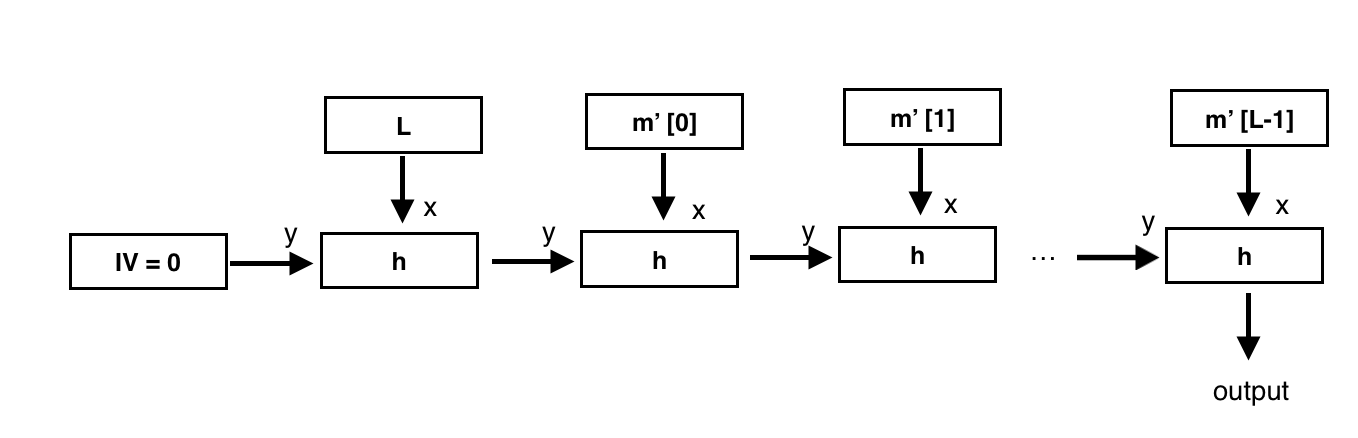
\includegraphics[width=15cm]{img/spcs-hash.png}
\end{center}

\subsection{}


Calculate the following using the PRP from section \ref{prp} and Davies-Meyer as $h$:

\begin{itemize}
\item $SPCS\text{-}Hash({\tt 0})$ \sol{{\tt 111}}
\item $SPCS\text{-}Hash({\tt 1})$ \sol{{\tt 100}}
\item $SPCS\text{-}Hash({\tt 00})$ \sol{{\tt 001}}
\item $SPCS\text{-}Hash({\tt 000})$ \sol{{\tt 001}}
\item $SPCS\text{-}Hash({\tt 000~111})$ \sol{{\tt 110}}
\item $SPCS\text{-}Hash({\tt 101~101})$ \sol{{\tt 001}}
\end{itemize}

\subsection{}

Since the PRP is very small, can you produce any collisions?

\newpage
\section{Compression Functions}

\subsection{Collision Resistance}

 
In class we saw that Davies-Meyer is often used to convert an ideal block cipher into a collision resistant compression function from 2 blocks to 1. Let $E(k,m)$ be a block cipher where the message space is the same as the key space (e.g. 128-bit AES). Show that the following methods do not work, by breaking the following:

\begin{itemize}
\item Collision Resistance: it's hard to find two different pairs of inputs $(x, y)$ and $(x', y')$ such that $h(x, y) = h(x', y')$.
\end{itemize}

First show how to do this in general (e.g. how you would do it for AES), then construct actual collisions using our block cipher.

\begin{itemize}
\item $h_1(x, y) = E(x, y) \oplus x$
\item $h_2(x, y) = E(y, x) \oplus y$
\item $h_3(x, y) = E(x, x \oplus y)$
\item $h_4(x, y) = E(x, x) \oplus x \oplus y$
\end{itemize}

(For the \emph{pair} to be different, you need either $x \neq x'$, or $y \neq y'$. If both are different, that also works.)

\sol{
This is from CS255 homeworks.


\begin{itemize}
\item $z, x = anything$, $y = D(x, x \oplus z)$
\item $z, y = anything$, $x = D(y, y \oplus z)$
\item $z, x = anything$, $y = D(x, z) \oplus x$
\item $z, x = anything$, $y = E(x, x) \oplus x$
\end{itemize}

For any of these: Choose two different values of ``anything'' to get a collision.

}

\subsection{Preimage Resistance}

Suppose someone gives you a specific target hash value $z$ (say, $z = 111...1$). For which of the previous compression functions can you find inputs $(x, y)$ such that $f(x, y) = z$?

\sol{
TOdO: Switch with previous question.
}

\newpage
\section{Breaking CBC-MAC as a Hash}

In class, we discussed how you can't convert CBC-MAC into a hash function because it wouldn't have pre image resistance and collision resistance.

Suppose we selected two values $k_1, k_2$ (permanently) and used the following hash:

$$
H : \{0, 1\}^* \to \{0, 1\}^n
$$


$$
H(x) = CBC\text{-}MAC\Big((k_1, k_2), pad(x)\Big)
$$


Show that it easy to break preimage resistance and collision resistance by finding expressions to calculate the following (for any choice of keys):

\begin{itemize}
\item Given $z$, show that you can find a message $x$ such that $H(x) = z$
\item Show that you can find messages $x, y$ such that $H(x) = H(y)$
\end{itemize}

Apply your answers $H(x)$ using our block cipher, with $k_1 = {\tt 001}$ and $k_2 = {\tt 010}$




\newpage
\section{Merkle Hash Trees}


Back in the day, Merkle suggested a parallel method for constructing hash functions out of compression functions. Let f be a compression function that takes two $n$-bit blocks and outputs one $n$-bit block. To hash a message $m$ we use the following tree construction:

\begin{center}
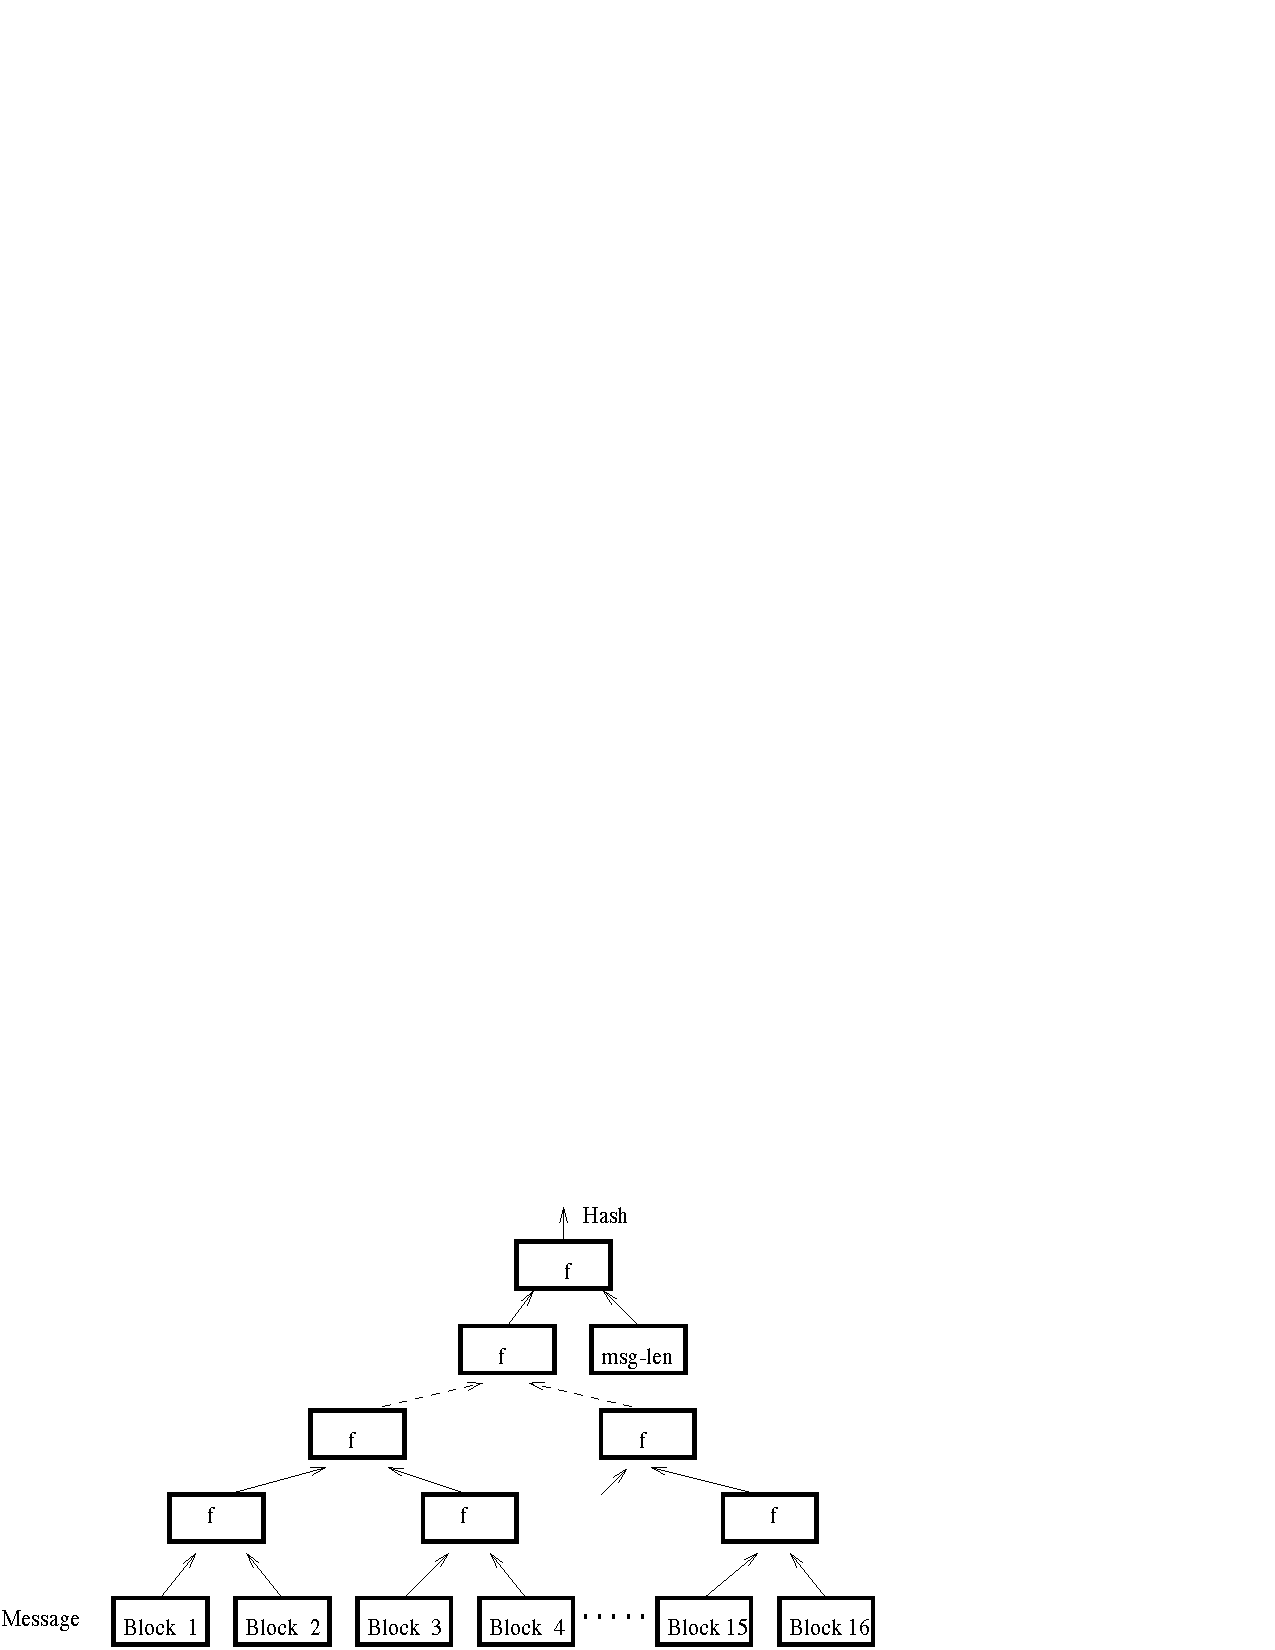
\includegraphics[width=10cm]{img/hash-tree.pdf}
\end{center}

For simplicity, assume that the number of blocks in $m$ is always a power of 2.

\subsection{}

Evaluate $H({\tt 000~001~010~011})$ using our PRP.


\sol{
${\tt 000}$
}

\subsection{}

\begin{itemize}
\item Prove that if one can find a collision for the resulting hash function then one can
find collisions for the compression function.
\item Show that if the msg-len block is eliminated (e.g. the contents of that block is always set to 0) then the construction is not collision resistant.
\end{itemize}

\sol{This is from CS255 homeworks.}

\subsection{}
Can you find a way to extend this to handle messages of arbitrary length? You will need to:

\begin{itemize}
\item Handle padding.
\item Prove that it is impossible to find any hash collisions if without finding collisions in the compression function.
\end{itemize}

(This is actually tricky to get right, and it's it's easy to believe your proof is your correct even if it has a significant mistake. I suggest you leave this question for the end.)



\section{Algorithm Substitution Attack}

Suppose we are having a secret communication using a key $m$, and want to allow someone with a certain master key $mk$ to listen in. Consider the following (authenticated) encryption algorithm $E_{PRP}(k, m)$ that uses a PRP $E$:

\begin{itemize}
\item Calculate $IV = E_{PRP}(mk, k)$
\item Send the usual (authenticated) encryption $AE(k, m)$, using the IV from the previous step.
\end{itemize}

Answer:

\begin{itemize}
\item Show that anyone with the master key can decrypt the message.
\item Show that the receiver (who also has $k$) can't tell the message apart from a valid encryption that uses a random IV.
\item Show that no one without either $k$ or $mk$ can decrypt the message.
\item What happens if you send the encryption of two different messages? Can you find a fix to the problem that comes up?
\end{itemize}

%
%\section{}
%
%Show that we can use an existing function $H : \{0, 1\}^* \to \{0, 1\}^128$ to create a hash function that maps values into $Z_p$ (assuming $p < 2^128$):
%
%$H : \{0, 1\}^* \to \Z_p$
%
%Hint: View the values in $\Z_p$ as binary strings in $\{0, 1\}^{128}$
%
%
%\section{Time-space tradeoff}
%Let $H : \mathcal{X} \to \mathcal{X}$ be a one-way permutation. Show that
%one can build a table $T$ of size $B$ bytes (where $B$ is a lot smaller than $|\mathcal{X}$) that enables an attacker to invert $f$ in using about time $|X|/B$ steps.. More precisely, construct an algorithm that takes as input the table $T$ and a $z \in \mathcal{X}$, and outputs an $x \in \mathcal{X}$ such that $H(x) = z$
%
%
%Hint: Pick a random point $a \in \mathcal{X}$ and compute the sequence
%\begin{itemize}
%\item $a_0 = a$
%\item $a_1 = H(a_0) = H(a)$
%\item $a_2 = H(a_1) = H(H(a))$
%\item $a_3 = H(a_2) = H(H(H(a)))$
%\item $a_4 = H(a_3) = H(H(H(H(a))))$
%\end{itemize}
%
%Since $H$ is a permutation, this sequence must come back to $a$ at some point (i.e. there
%is some $j > 0$ such that $a_j = a$). We call the resulting sequence$ (a_0, a1, . . . , a_j)$ an
%$H$-cycle. Let $t = |X|/B$ (rounded up). Try storing $(z_0, z_t, z_{2t}, z_{3t}, ...)$ in a table. 
%(or perhaps, several such tables) to invert an input $x \in \mathcal{X}$ in about $t$ steps.
%



\end{document}
